% !TeX program = xelatex
% !TeX spellcheck = en_GB
\documentclass[11pt]{beamer}

%-------------------------------------------------------
% THEMES, COLORS
%-------------------------------------------------------
%\usetheme{Warsaw}
%\usetheme{Baodilla}
%\usetheme{CambridgeUS}
%\usetheme{AnnArbor}
%\usecolortheme{beaver}
%\usetheme{Madrid}

\usefonttheme{professionalfonts}
\usepackage{amsmath,mathtools,bm}
\usepackage{xcolor}
\usepackage{rotating,graphicx}

%--------------------------------------------------------
% COLOR DEFINITIONS
%---------------------------------------------------------
\definecolor{amber}{rgb}{1.0, 0.49, 0.0}
\definecolor{olivedrab}{rgb}{0.42, 0.56, 0.14}
\definecolor{darkolivegreen}{rgb}{0.33, 0.42, 0.18}
\definecolor{chromeyellow}{rgb}{1.0, 0.65, 0.0}
\definecolor{beige}{rgb}{0.96, 0.96, 0.86}
\definecolor{bluegreen}{rgb}{3, 166, 155}
\definecolor{pitchblack}{rgb}{0, 0, 0}
\definecolor{lightbeige}{rgb}{255, 251, 241}
\definecolor{mediumgray}{rgb}{183, 183, 183}
\definecolor{carrotorange}{rgb}{0.93, 0.57, 0.13}
\definecolor{orange-red}{rgb}{1.0, 0.27, 0.0}
\definecolor{ferngreen}{rgb}{0.31, 0.47, 0.26}
\definecolor{darkspringgreen}{rgb}{0.09, 0.45, 0.27}
\definecolor{cocoabrown}{rgb}{0.82, 0.41, 0.12}
\definecolor{darkorange}{rgb}{1.0, 0.55, 0.0}
\definecolor{deepcarrotorange}{rgb}{0.91, 0.41, 0.17}
%---------------------------------------------------------

%-------------------------------------------------------------------------
% NEW THEME
%-------------------------------------------------------------------------
%\usetheme{Frankfurt}
\usetheme{Madrid}
\definecolor{UBCblue}{rgb}{0.04706, 0.13725, 0.26667} % UBC Blue (primary)
\definecolor{UBCgrey}{rgb}{0.3686, 0.5255, 0.6235} % UBC Grey (secondary)

%\useoutertheme{infolines} % Alternatively: miniframes, infolines, split
%\useinnertheme{circles}
%
%\usecolortheme[named=UBCblue]{structure}
%\setbeamercolor{palette primary}{bg=UBCblue,fg=white}
%\setbeamercolor{palette secondary}{bg=UBCblue,fg=white}
%\setbeamercolor{palette tertiary}{bg=UBCblue,fg=white}
%\setbeamercolor{palette quaternary}{bg=UBCblue,fg=white}
%\setbeamercolor{structure}{fg=UBCblue} % itemize, enumerate, etc
%\setbeamercolor{section in toc}{fg=UBCblue} % TOC sections
%
%% Override palette coloring with secondary
%\setbeamercolor{subsection in head/foot}{bg=UBCgrey,fg=white}
%---------------------------------------------------------------------------

%\setbeamercolor{background canvas}{bg=pitchblack}
%\setbeamercolor{normal text}{fg=beige}
%\setbeamercolor{frametitle}{bg=pitchblack, fg=chromeyellow}
%\setbeamercolor{headline}{bg=pitchblack, fg=chromeyellow}
%\setbeamercolor{item projected}{bg=chromeyellow}
%\setbeamertemplate{enumerate items}[default]
%\setbeamertemplate{navigation symbols}{}
%\setbeamercovered{transparent}
%\setbeamercolor{block title}{fg=chromeyellow}
%\setbeamercolor{local structure}{fg=chromeyellow}

%-------------------------METRONOM THEME---------------------------------------

\usepackage{textpos} % Required to position Metronom logo

\useoutertheme{infolines} % Alternatively: miniframes, infolines, split
\useinnertheme{circles}

\usecolortheme[named=pitchblack]{structure}
\setbeamercolor{palette primary}{bg=pitchblack,fg=chromeyellow}
\setbeamercolor{palette secondary}{bg=pitchblack,fg=chromeyellow}
\setbeamercolor{palette tertiary}{bg=pitchblack,fg=chromeyellow}
\setbeamercolor{palette quaternary}{bg=pitchblack,fg=chromeyellow}
\setbeamercolor{structure}{fg=pitchblack} % itemize, enumerate, etc
\setbeamercolor{section in toc}{fg=pitchblack} % TOC sections

% Override palette coloring with secondary
\setbeamercolor{subsection in head/foot}{bg=pitchblack,fg=white}

% Add logo
%\addtobeamertemplate{footline}{}{%
%\begin{textblock*}{100mm}(.82\textwidth,-1cm)
%\includegraphics[scale=0.025]{Metronom}
%\end{textblock*}}

%\setbeamertemplate{background canvas}{%
%   \begin{picture}(0,0)
%     \put(10,10){\includegraphics[scale=0.1]{Metronom}}
%   \end{picture}
%}%
%-----------------------------------------------------------------------------

%-----------------------------------------------------------------------------
% FONT PACKAGES
%-----------------------------------------------------------------------------

\usepackage[utf8]{inputenc}
\usepackage[english]{babel}
\usepackage[T1]{fontenc}
\usepackage{fontspec}
%\usepackage{helvet}
%-------------------------------------------------------
% DEFFINING AND REDEFINING COMMANDS
%-------------------------------------------------------
\newcommand{\R}{\ensuremath{\mathbf{R}}}
\newcommand{\html}[1]{\texttt{\detokenize{#1}}}
%-------------------------------------------------------
% INFORMATION IN THE TITLE PAGE
%-------------------------------------------------------

\title[Universal Approximation]{A Visual Proof of the Universal Approximation
Theorem}


\author[Data Science]{Somnath Sikdar}
\date{\today}

\begin{document}
\maketitle

\begin{frame}[t]
\frametitle{Neurons and Neural Networks}
{\small
\begin{itemize}
    \item Neural networks are comprised of neurons.
    \item A single neuron can accept an arbitrary number of inputs
        $x_1, \ldots, x_k$.
\end{itemize}
}
\begin{minipage}[b]{0.25\textwidth}
\begin{center}
    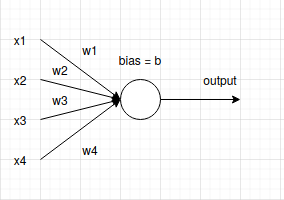
\includegraphics[scale=0.35]{singleNeuron.png}
\end{center}
\end{minipage}
\hfill
\begin{minipage}[b]{0.7\textwidth}
{\small
\begin{itemize}
    %\item Neural networks are comprised of neurons.
    %\item A single neuron can accept an arbitrary number of inputs
    %    $x_1, \ldots, x_k$.
    \item The output of a neuron is $\Psi(\sum_{i = 1}^{k} w_i x_i + b)$,
        where $w_1, \ldots, w_k$ are the input weights, $b$ is the bias
        and $\Psi$ is called the activation function.
    \item A typical activation function is the sigmoid function
        \[\sigma(x_1, \ldots, x_k) = \frac{1}{1 + e^{- (\sum_{i} w_i x_i + b)}}.\]
\end{itemize}
}
\end{minipage}
\end{frame}

\begin{frame}[t]
\frametitle{Feedforward Neural Networks}
\vspace{-1cm}
\begin{center}
\begin{turn}{-90}
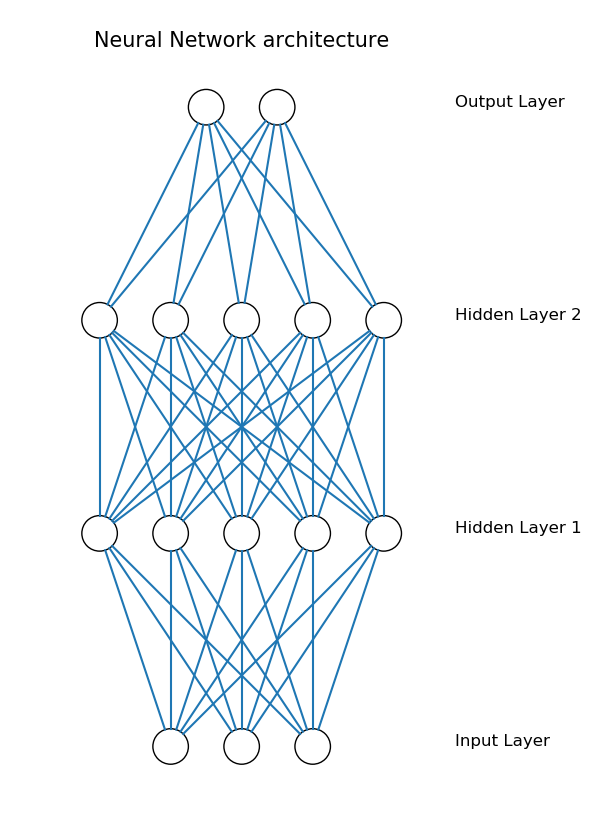
\includegraphics[scale=0.28]{feedforward.png}
\end{turn}
\end{center}
{\small
\begin{itemize}
    \item A network with $m$ input nodes and $n$ output
        neurons compute functions from $\R^m$ to $\R^n$.
    \item What is this class of functions?
\end{itemize}
}
\end{frame}



\begin{frame}[t,fragile]
\frametitle{The Universal Approximation Theorem}
{\small It turns out that:
\begin{quote}
Feedforward networks can compute any continuous function from $\R^m$
to $\R^n$ to any desired degree of accuracy.
\end{quote}

First shown by:
\begin{itemize}
    \item George Cybenko. \emph{Approximation by superpositions of a sigmoidal
        function}. Mathematics of Control, Signals and Systems, Volume 2, 1989.

    \item Kurt Hornik, Maxwell Stinchcombe, Halbert White. \emph{Multilayer
        feedforward networks are universal approximators}. Neural Networks,
        Volume 2, Issue 5, 1989.
\end{itemize}
Hornik et al.
\begin{quote}
 $\ldots$ that standard multilayer feedforward networks with as few as
one hidden layer using arbitrary squashing functions are capable of
approximating any Borel measurable function from one finite dimensional
space to another to any desired degree of accuracy, provided sufficiently
many hidden units are available.
\end{quote}
}
\end{frame}

\begin{frame}[t,fragile]
\frametitle{What we will show}
{\small
Feedforward networks with
\begin{itemize}
    \item two hidden layers with sigmoid neurons
    \item an output layer with linear neurons
\end{itemize}
can approximate any continuous function from one real vector space
to another.

\medskip
\textbf{Comparison with Hornik et al.}
\begin{itemize}
    \item Continuous functions are Borel functions but not all
        Borel functions are continuous.
    \item Any activation function $\Psi \colon \R \to [0, 1]$
        that is non-decreasing with $\lim_{x \to \infty} \Psi (x)= 1$ and
        $\lim_{x \to -\infty} \Psi (x) = 0$ will do. Can have countably
        many discontinuities.
    \item \textbf{One} hidden layer with activation functions and the output layer
        with neurons with a linear activation.
\end{itemize}
}
\end{frame}

\begin{frame}[t]
\frametitle{Single Sigmoid Neurons}
{\small
\[
    \sigma (x) = \frac{1}{1 + e^{-(w x + b)}}.
\]
\begin{center}
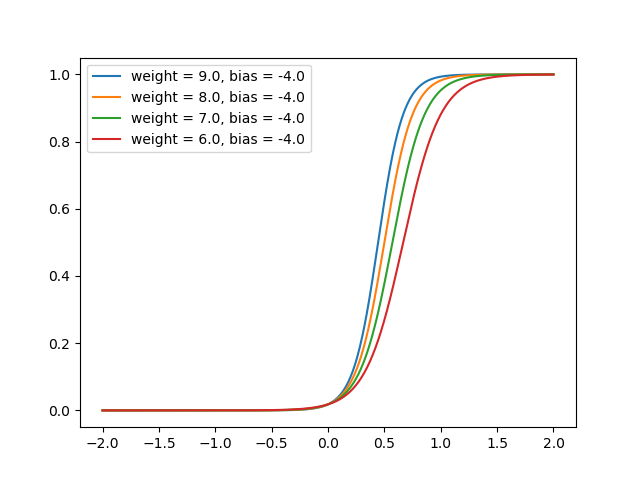
\includegraphics[scale=0.4]{sigmoidOutput.png}
\end{center}
\begin{itemize}
    \item The sigmoid squishes values to the interval $[0, 1]$.
    \item At the point $- b / w$, the function attains the value $1/2$.
\end{itemize}
}
\end{frame}

\begin{frame}[t]
\frametitle{Using Sigmoid Neurons to Approximate Step Functions}
{\small
If we use a large enough weight, then at the point $- b / w$, we can
cause the function to step up from $0$ to $1$.
\begin{center}
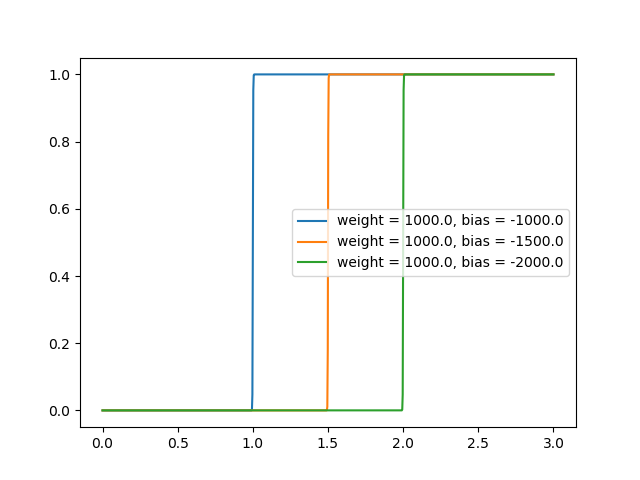
\includegraphics[scale=0.4]{stepfunction.png}
\end{center}
}
\end{frame}

\begin{frame}[t]
\frametitle{From Step to Rectangle Functions}
\begin{center}
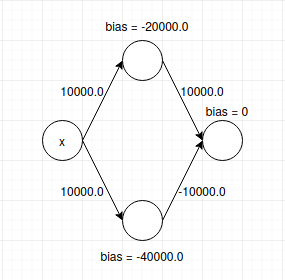
\includegraphics[scale=0.3]{nnRectangleFunction.png}
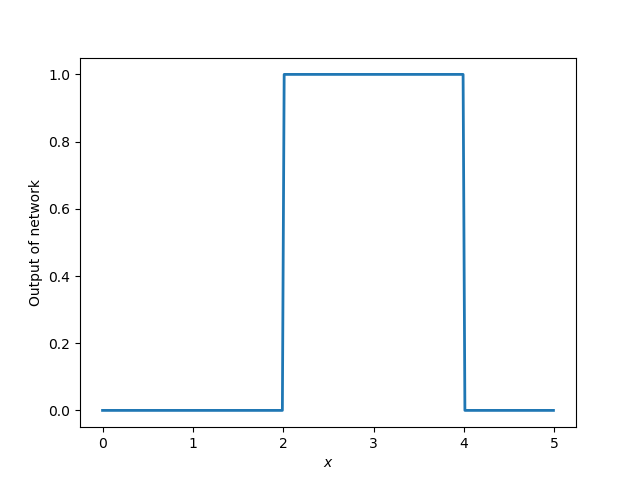
\includegraphics[scale=0.35]{xStepFunction.png}
\end{center}
\end{frame}

\begin{frame}[t]
\frametitle{Code for the Rectangle Function}
\begin{minipage}[b]{0.4\textwidth}
\begin{center}
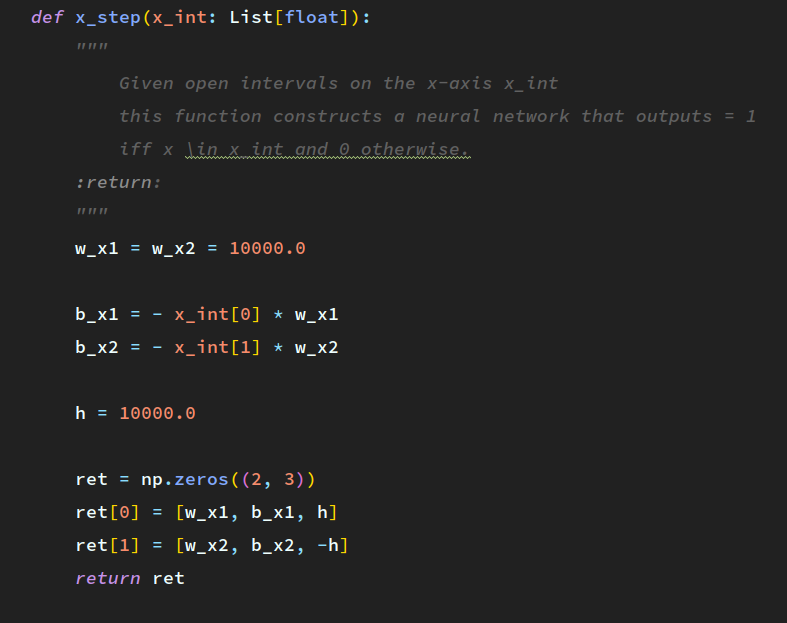
\includegraphics[scale=0.25]{codeRectangleFunction.png}
\end{center}
\end{minipage}
\hspace{0.5cm}
\begin{minipage}[b]{0.4\textwidth}
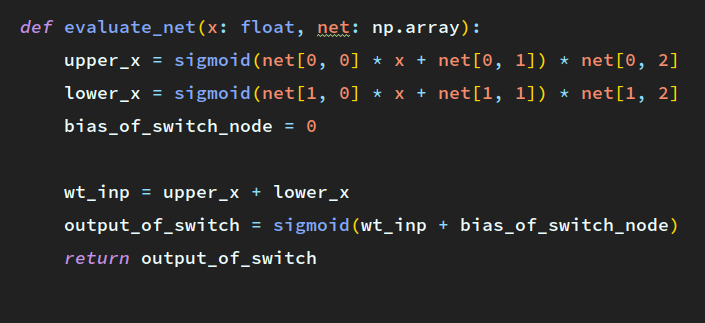
\includegraphics[scale=0.25]{codeEvaluateRectangleFunction.png}
\end{minipage}
\end{frame}

\begin{frame}[t]
\frametitle{From Rectangle Functions to Univariate Functions}
\begin{minipage}[b]{0.3\textwidth}
\begin{center}
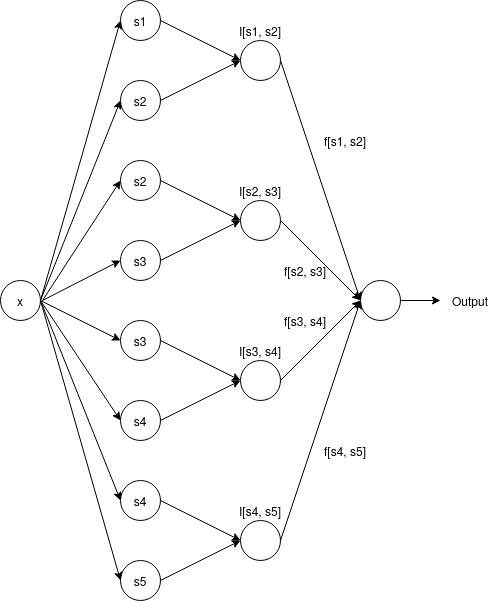
\includegraphics[scale=0.3]{OneVariableFunctions.jpg}
\end{center}
\end{minipage}
\hfill
\begin{minipage}[b]{0.5\textwidth}
{\small
\begin{itemize}
    \item The output neuron has a linear activation.
    \item Hidden layers have only sigmoid neurons.
    \item When $x \in [s_i, s_{i + 1}]$ for $i \in \{1, 2, 3, 4\}$,
        the corresponding sub-network $I[s_1, s_{i + 1}]$ outputs a $1$;
        all other sub-networks output $0$.
    \item The final output of the network is then $f[s_i, s_{i + 1}]$,
        the approximate value of $f$ in this interval.
\end{itemize}
}
\end{minipage}
\end{frame}

\begin{frame}[t]
\frametitle{From Rectangle Functions to Univariate Functions}
{\small $ f(x) = 0.2 + 0.4 x^2 + 0.3 x \sin(15 x) + 0.05 \cos(50 x)$}
\begin{center}
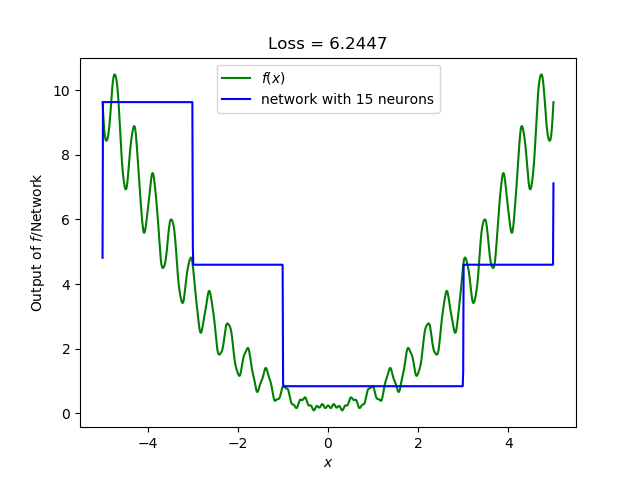
\includegraphics[scale=0.28]{5IntervalApprox.png}
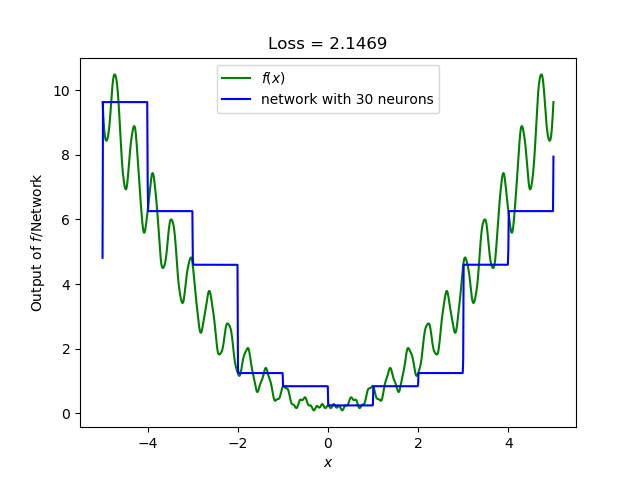
\includegraphics[scale=0.28]{10IntervalApprox.png}
\end{center}
\vspace{-0.5cm}
\begin{center}
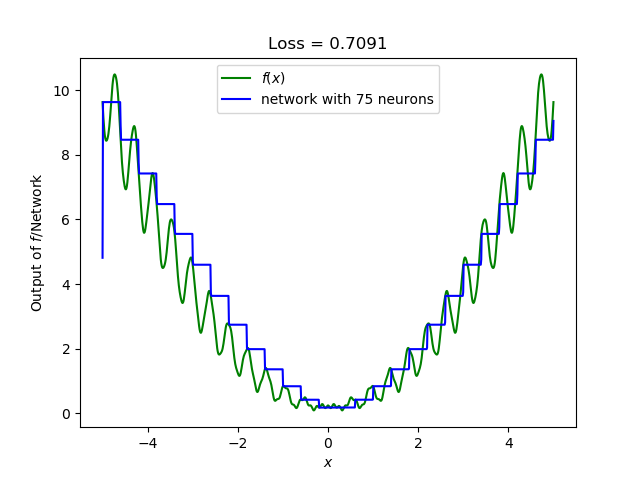
\includegraphics[scale=0.28]{25IntervalApprox.png}
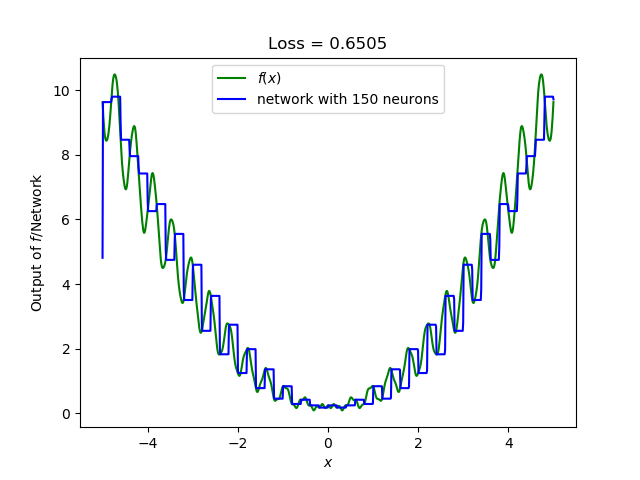
\includegraphics[scale=0.28]{50IntervalApprox.png}
\end{center}
\end{frame}

\begin{frame}[t]
\frametitle{From Univariate to Bivariate Functions}
Generalize rectangle functions in the 2D plane:
\begin{minipage}{0.4\textwidth}
\begin{center}
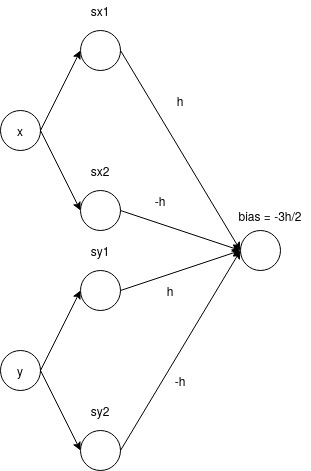
\includegraphics[scale=0.3]{nnTowerFunction.jpg}
\end{center}
\end{minipage}
\hfill
\begin{minipage}{0.5\textwidth}
\begin{center}
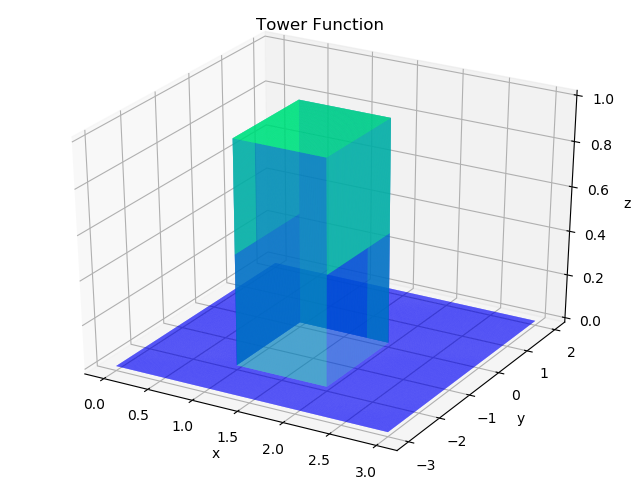
\includegraphics[scale=0.3]{TowerFunction.png}
\end{center}
\end{minipage}
{\small
\begin{itemize}
    \item $s_x = [1.0, 2.0]; s_y = [-2.0, -0.0]$;
    \item $w_{x1} = w_{x2} = w_{y1} = w_{y2} = 100000.0$;
    \item $b_{x1} = -100000.0$; $b_{x2} = -200000.0$; $b_{y1} = 200000.0$; $b_{y2} = 0.0$;
    \item $h = 10000.0$
\end{itemize}
}
\end{frame}

\begin{frame}[t]
\frametitle{Code for the Tower Function}
\begin{center}
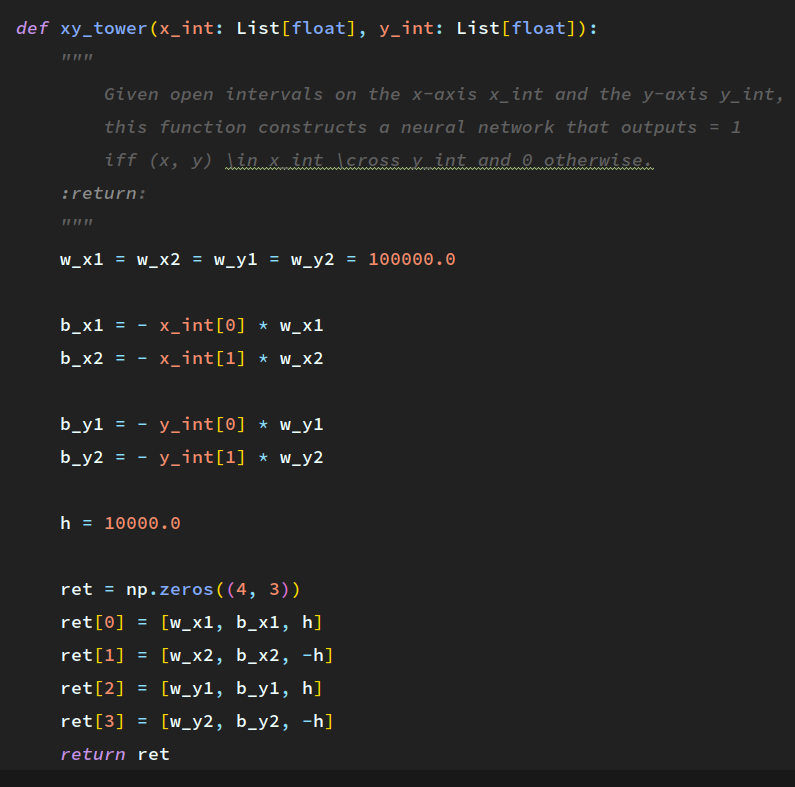
\includegraphics[scale=0.25]{codeXYTower.png}
\end{center}
\end{frame}

\begin{frame}[t]
\frametitle{Generalizing to Multivariate Functions}
{\small
\begin{itemize}
    \item A function $f$ from $\R^m$ to $\R^n$ can be decomposed into $n$ functions
          $f_1(x_1, \ldots, x_m), \ldots, f_n(x_1, \ldots, x_m)$ from $\R^m \to \R^1$.
    \item Hence this case can be handled by combining $n$ networks, one for each
        of the $n$ functions.
\end{itemize}
}
\end{frame}

\begin{frame}[t]
\frametitle{Code, References}
{\small
All code available at:
\begin{itemize}
    \item \html{https://github.com/somnath1077/MachineLearningExercises/}
          \html{tree/master/NN_DeepLearning/other_code}
\end{itemize}

\bigskip

\textbf{References}

\begin{itemize}
    \item Michael Nielsen. Neural Networks and Deep Learning, Chapter~$4$. Available at:
    \html{http://neuralnetworksanddeeplearning.com/}
\end{itemize}
}
\end{frame}
\end{document}
